
\begin{frame}[ctb!]
  \frametitle{Resource Exchange Generality}

  To determine a supply-demand resource exchange for \textit{general} facilities
  in the fuel cycle, detailed information about both the supply and demand must
  be known.

  Some examples:
  
  \begin{itemize}
    \item Enrichment facilities - constrained by both quality and quantity of fuel
      requested
    \item Reactors - request specific isotopic profiles for new fuel
    \item Fabrication facilities - must know the isotopic profile of fuel to
      provide
  \end{itemize}
  
\end{frame}

\begin{frame}[ctb!]
  \frametitle{Resource Exchange Information Gathering}

  The nuclear fuel cycle has some similarities to the petroleum industry (i.e.,
  the quality of the product must be taken into account), and is a
  \textit{supply chain}.\\

  Furthermore, facilities making decisions based on product quality act in an
  agent-like manner.\\ 

  Accordingly, I looked toward agent-based supply chain modeling of the
  petroleum industry for inspiration, and have adopted an approach proposed by
  Julka et. al \cite{julka_agent-based_2002} to be used under the proposed
  \Cyclus design constraints.
\end{frame}

\begin{frame}[ctb!]
  \frametitle{Resource Exchange: Request for Bids}
  \begin{figure}
    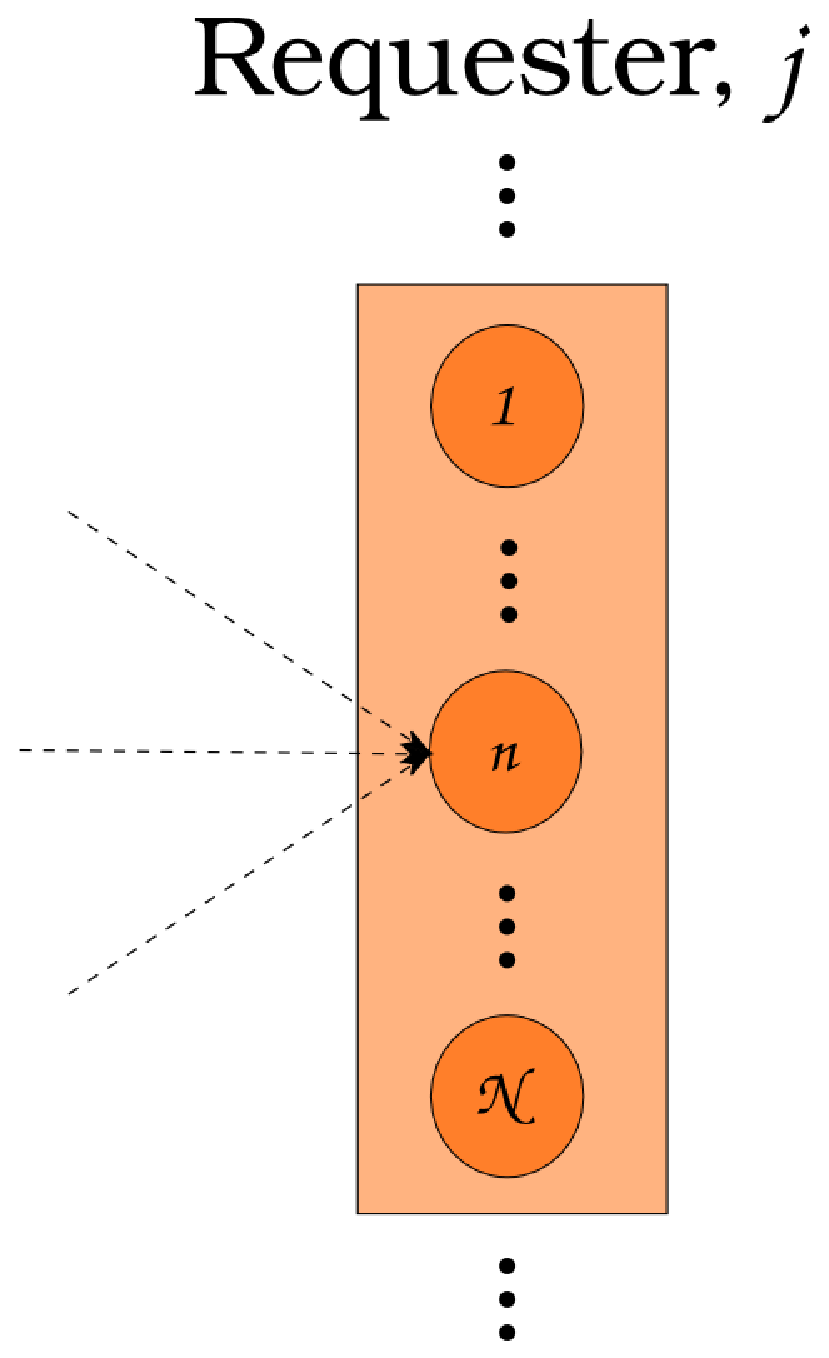
\includegraphics[height=5cm]{./images/requester.eps}
    \caption{Consumers define their demand for commodities during the Request
      for Bids (RFB) phase.}
  \end{figure}
\end{frame}

\begin{frame}[ctb!]
  \frametitle{Resource Exchange: Response to Request for Bids}
  \begin{figure}
    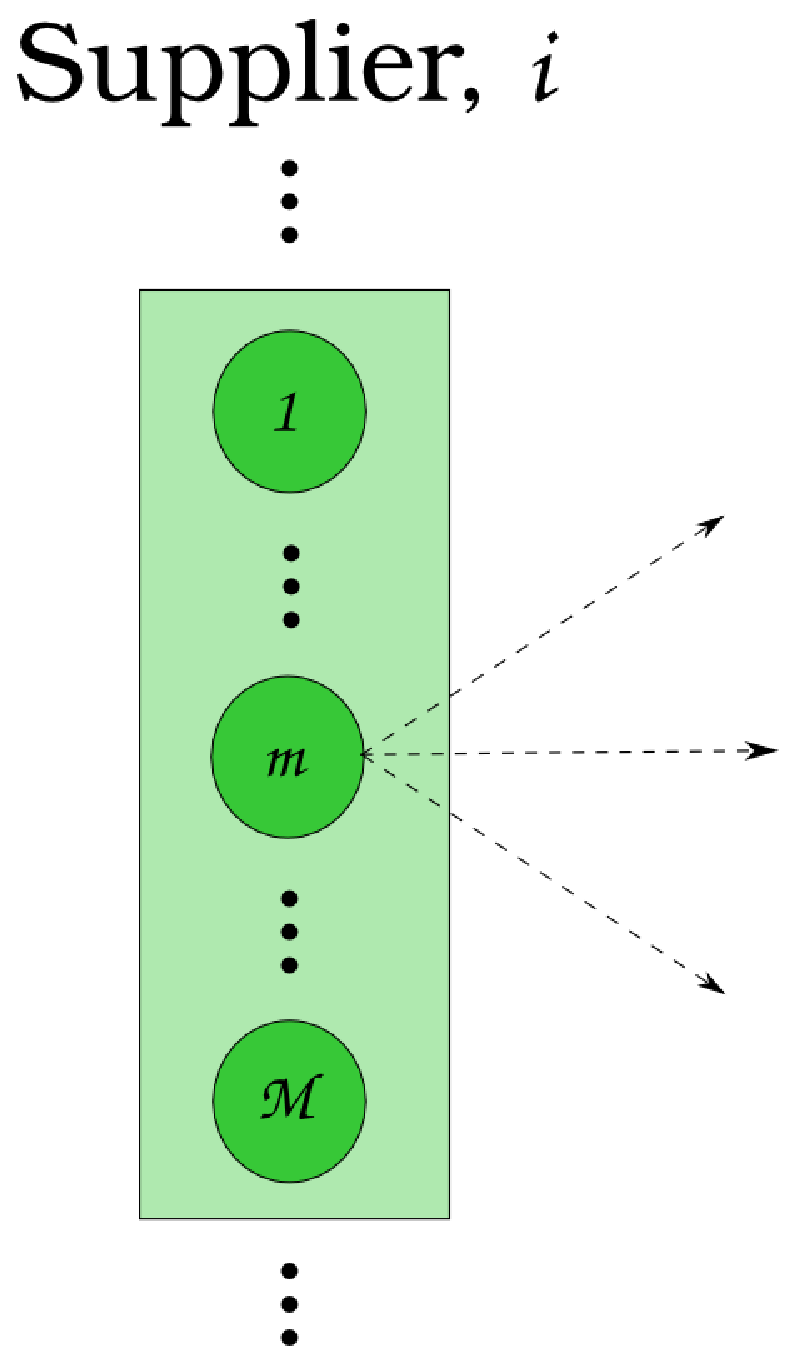
\includegraphics[height=5cm]{./images/supplier.eps}
    \caption{Suppliers respond to each request during the Response to Request
      for Bids (RRFB) phase.}
  \end{figure}
\end{frame}

\begin{frame}[ctb!]
  \frametitle{Resource Exchange: Preference Adjustment}
  \begin{figure}
    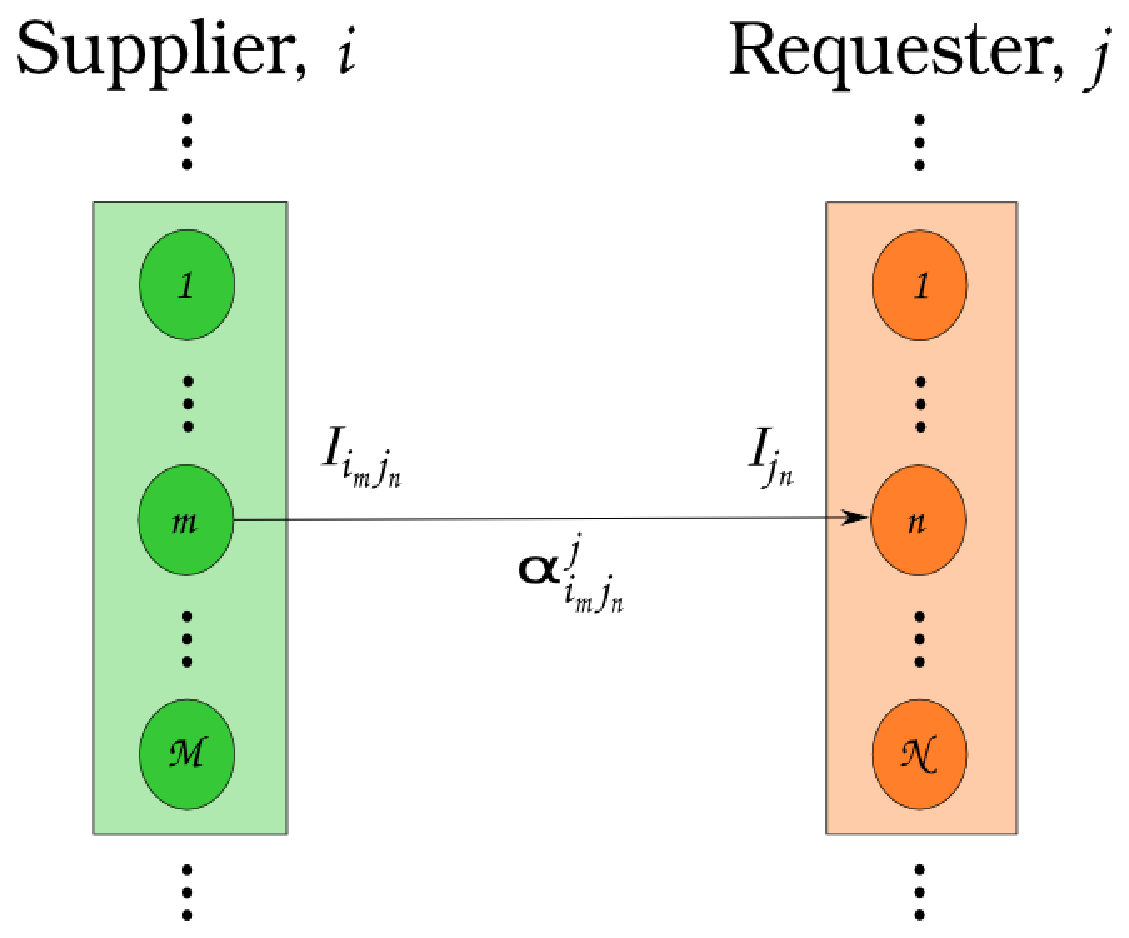
\includegraphics[height=5cm]{./images/supplier-requester.eps}
    \caption{Consumers adjust preferences based on Supplier-given information
      during the Preference Adjustment (PA) phase.}
  \end{figure}

  Managers of facilities (institutions, regions) are then allowed to perturb
  preferences.
\end{frame}

\begin{frame}[ctb!]
  \frametitle{Resource Exchange: Full Picture}
  \begin{figure}
    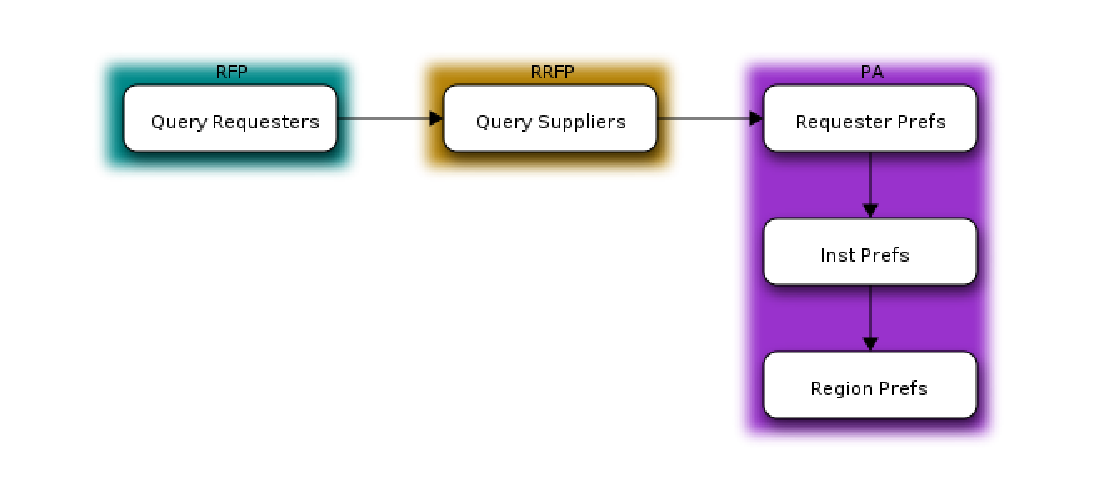
\includegraphics[height=5cm]{./images/exchange.eps}
    \caption{A flow chart of the information gathering phases.}
  \end{figure}
\end{frame}

\begin{frame}[ctb!]
  \frametitle{Resource Exchange Solution Mechanism}
  
  As defined, facilities in \Cyclus are black boxes, but there is a notion of
  supplier and consumer facilities of a variety of commodities.\\

  We seek a solution to a flow of (discrete) materials, where for each
  commodity, we have now defined a set of suppliers and consumers of that
  commodity.\\ 
  
  Furthermore, suppliers may be able to provide more than one commodity and
  consumers may be able to consume more than one commodity.\\

  Accordingly, a Multicommodity Transportation Problem formulation naturally
  fits the needs of our simulation. Let's call it the Generic Fuel Cycle
  Transportation Problem (GFCTP).
  
\end{frame}


\begin{frame}[ctb!]
  \frametitle{GFCTP - Description}

  here we are
  
\end{frame}
